% generated by doc/figures.py -- edit the script, not this file
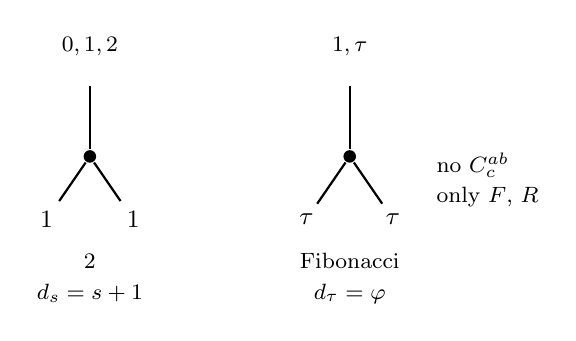
\begin{tikzpicture}[thick, every node/.style={font=\small}]
  % SU(2): 1 (x) 1 = 0 + 1 + 2
  \node (l1) at (0,0) {$1$};
  \node (l2) at (1.1,0) {$1$};
  \node[circle, fill, inner sep=1.6pt] (v) at (0.55,0.8) {};
  \draw (l1) -- (v); \draw (l2) -- (v);
  \draw (v) -- (0.55,1.7);
  \node[align=left] at (0.55,2.2) {\footnotesize $0,1,2$};
  \node[align=center] at (0.55,-0.75)
    {\footnotesize $\SU{2}$\\ \footnotesize $d_s=s+1$};
  \node at (2.0,0.8) {$\quad$};
  % Fibonacci: tau (x) tau = 1 + tau
  \node (m1) at (3.3,0) {$\tau$};
  \node (m2) at (4.4,0) {$\tau$};
  \node[circle, fill, inner sep=1.6pt] (w) at (3.85,0.8) {};
  \draw (m1) -- (w); \draw (m2) -- (w);
  \draw (w) -- (3.85,1.7);
  \node[align=left] at (3.85,2.2) {\footnotesize $1,\tau$};
  \node[align=center] at (3.85,-0.75)
    {\footnotesize Fibonacci\\ \footnotesize $d_\tau=\varphi$};
  \node[align=left] at (5.6,0.5)
    {\footnotesize no $C^{ab}_{c}$\\ \footnotesize only $F$, $R$};
\end{tikzpicture}
